\documentclass{article}
\usepackage{graphicx}
\usepackage{listings}
\usepackage{xcolor}
\usepackage{amsmath}
\usepackage[a4paper, margin=1in]{geometry}
\setlength{\parindent}{0pt}

\title{Bitonic Sort Report}
\author{111062117, Hsiang-Sheng Huang}

\begin{document}

\maketitle


\section*{Implementation Overview}
\subsection*{Local Bitonic Sort}
\begin{lstlisting}[language=C++, basicstyle=\ttfamily\small, keywordstyle=\color{blue}\bfseries, commentstyle=\color{gray}\itshape, stringstyle=\color{red}, numbers=left, numberstyle=\tiny\color{gray}, stepnumber=1, frame=single, showstringspaces=false, breaklines=true]
void compSwap(float &a, float &b, bool dir) {
  if ((a > b) == dir) swap(a, b);
}

void bitonic_sort_loop(vector<float>& arr) {
  const int n = (int)arr.size();  // n must be 2^k
  for (int k = 2; k <= n; k <<= 1)
    for (int j = k >> 1; j > 0; j >>= 1)
      for (int i = 0; i < n; ++i) {
        int ixj = i ^ j;
        if (ixj > i) {
          bool dir = ((i & k) == 0);  // true=ASC, false=DESC
          compSwap(arr[i], arr[ixj], dir);
        }
      }
}
\end{lstlisting}

Each MPI \emph{rank} first performs a \textbf{local} bitonic sort on its private segment. I chose the iterative variant to avoid extra call-stack overhead incurred by the recursive implementation.

\paragraph{Time Complexity}
The three nested loops yield $k = \log_2 n$, $j = \log_2 n$, and $i = n$ iterations, giving
$\mathcal{O}(n\log^2 n)$.

\subsection*{Parallel Bitonic Merge}
After every rank holds a locally sorted block, we repeatedly compare-exchange with a partner rank so that, after $\log_2 p$ phases, the global order is established.

\subsubsection*{Merging the High / Low Halves}
\begin{lstlisting}[language=C++, basicstyle=\ttfamily\small, keywordstyle=\color{blue}\bfseries, commentstyle=\color{gray}\itshape, stringstyle=\color{red}, numbers=left, numberstyle=\tiny\color{gray}, stepnumber=1, frame=single, showstringspaces=false, breaklines=true]
void merge_high(const vector<float>& a, const vector<float>& b, vector<float>& res, int n) {
  int j = n - 1, k = n - 1;
  for (int i = n - 1; i >= 0; --i) {
    if (j < 0) res[i] = b[k--];
    else if (k < 0) res[i] = a[j--];
    else if (a[j] > b[k]) res[i] = a[j--];
    else res[i] = b[k--];
  }
}

void merge_low(const vector<float>& a, const vector<float>& b, vector<float>& res, int n) {
  int j = 0, k = 0;
  for (int i = 0; i < n; ++i) {
    if (j >= n) res[i] = b[k++];
    else if (k >= n) res[i] = a[j++];
    else if (a[j] < b[k]) res[i] = a[j++];
    else res[i] = b[k++];
  }
}
\end{lstlisting}

The \texttt{merge\_high} routine keeps the larger half (descending), while \texttt{merge\_low} keeps the smaller half (ascending).

\subsubsection*{Stable Tag Generation}
We use the Cantor pairing function to generate unique MPI tags:
\[
\text{cantor}(a,b) \;=\; \frac{(a+b)(a+b+1)}{2} + b.
\]

\subsubsection*{Compare-Exchange Kernel}
\begin{lstlisting}[language=C++, basicstyle=\ttfamily\small, keywordstyle=\color{blue}\bfseries, commentstyle=\color{gray}\itshape, stringstyle=\color{red}, numbers=left, numberstyle=\tiny\color{gray}, stepnumber=1, frame=single, showstringspaces=false, breaklines=true]
void cmp(vector<float>& local, int localN, int partner, bool dir, MPI_Comm comm) {
  int rank;
  MPI_Comm_rank(comm, &rank);

  MPI_Request req[2];
  MPI_Status stat[2];

  int cantor_arg1 = (dir == true) ? rank : partner;
  int cantor_arg2 = (dir == true) ? partner : rank;
  int send_tag = (1 + (dir == true)) * cantor(cantor_arg1, cantor_arg2);
  int recv_tag = (1 + (dir == false)) * cantor(cantor_arg1, cantor_arg2);

  vector<float> recv(localN);
  if (dir == true) {
    MPI_Isend(local.data(), localN, MPI_FLOAT, partner, send_tag, comm, &req[0]);
    MPI_Irecv(recv.data(), localN, MPI_FLOAT, partner, recv_tag, comm, &req[1]);
  } else {
    MPI_Irecv(recv.data(), localN, MPI_FLOAT, partner, recv_tag, comm, &req[0]);
    MPI_Isend(local.data(), localN, MPI_FLOAT, partner, send_tag, comm, &req[1]);
  }

  MPI_Waitall(2, req, stat);

  vector<float> res(localN);
  if (dir == true) merge_low(local, recv, res, localN);
  else merge_high(local, recv, res, localN);
  local.swap(res);
}
\end{lstlisting}

Here, \texttt{dir == true} means ascending order for the current exchange.

\subsection*{Main}
\begin{lstlisting}[language=C++, basicstyle=\ttfamily\small, keywordstyle=\color{blue}\bfseries, commentstyle=\color{gray}\itshape, stringstyle=\color{red}, numbers=left, numberstyle=\tiny\color{gray}, stepnumber=1, frame=single, showstringspaces=false, breaklines=true]
int p = __lg(usedP);
for (int i = 0; i < p; ++i)
  for (int j = i; j >= 0; --j) {
    int partner = rank ^ (1 << j);
    bool dir = ((rank >> (i + 1)) & 1) == ((rank >> j) & 1);
    cmp(local, localN, partner, dir, activeComm);
  }
\end{lstlisting}

The outer loop iterates over stages $i$, and the inner loop over levels $j$. Each rank communicates with exactly one partner per $(i,j)$.

\section*{Handling Non-Power-of-Two Cases}
\subsection*{Input Size $N \neq 2^k$}
Pad with $+\infty$ so extra elements bubble to the end:
\begin{lstlisting}[language=C++, basicstyle=\ttfamily\small, keywordstyle=\color{blue}\bfseries, commentstyle=\color{gray}\itshape, stringstyle=\color{red}, numbers=left, numberstyle=\tiny\color{gray}, stepnumber=1, frame=single, showstringspaces=false, breaklines=true]
int paddedN = 1;
while (paddedN < N) paddedN <<= 1;
// ...
vector<float> data;
data.resize(paddedN, numeric_limits<float>::infinity());
\end{lstlisting}

\subsection*{Processor Count $p \neq 2^k$}
Dismiss ranks beyond the largest power-of-two:
\begin{lstlisting}[language=C++, basicstyle=\ttfamily\small, keywordstyle=\color{blue}\bfseries, commentstyle=\color{gray}\itshape, stringstyle=\color{red}, numbers=left, numberstyle=\tiny\color{gray}, stepnumber=1, frame=single, showstringspaces=false, breaklines=true]
    int usedP = 1 << __lg(world_size);
int color = (world_rank < usedP) ? 0 : MPI_UNDEFINED;

MPI_Comm activeComm;
MPI_Comm_split(MPI_COMM_WORLD, color, world_rank, &activeComm);
if (color == MPI_UNDEFINED) {
  MPI_Finalize();
  return 0;
}
\end{lstlisting}

\section*{I/O Strategy}
Centralised I/O on rank 0:
\begin{lstlisting}[language=C++, basicstyle=\ttfamily\small, keywordstyle=\color{blue}\bfseries, commentstyle=\color{gray}\itshape, stringstyle=\color{red}, numbers=left, numberstyle=\tiny\color{gray}, stepnumber=1, frame=single, showstringspaces=false, breaklines=true]
if (rank == 0) {
  data.resize(paddedN, numeric_limits<float>::infinity());
  MPI_File inFH;
  MPI_File_open(MPI_COMM_SELF, inFile, MPI_MODE_RDONLY, MPI_INFO_NULL, &inFH);
  MPI_File_read_at(inFH, 0, data.data(), N, MPI_FLOAT, MPI_STATUS_IGNORE);
  MPI_File_close(&inFH);
}


MPI_Scatter(data.data(), localN, MPI_FLOAT, local.data(), localN, MPI_FLOAT, 0, activeComm);
// ...
if (rank == 0) {
  ans.resize(N);
  MPI_File outFH;
  MPI_File_open(MPI_COMM_SELF, outFile, MPI_MODE_CREATE | MPI_MODE_WRONLY, MPI_INFO_NULL, &outFH);
  MPI_File_write_at(outFH, 0, ans.data(), N, MPI_FLOAT, MPI_STATUS_IGNORE);
  MPI_File_close(&outFH);
}
\end{lstlisting}

\section*{Experimental Results (IPM)}
\begin{figure}[h!]
    \centering
    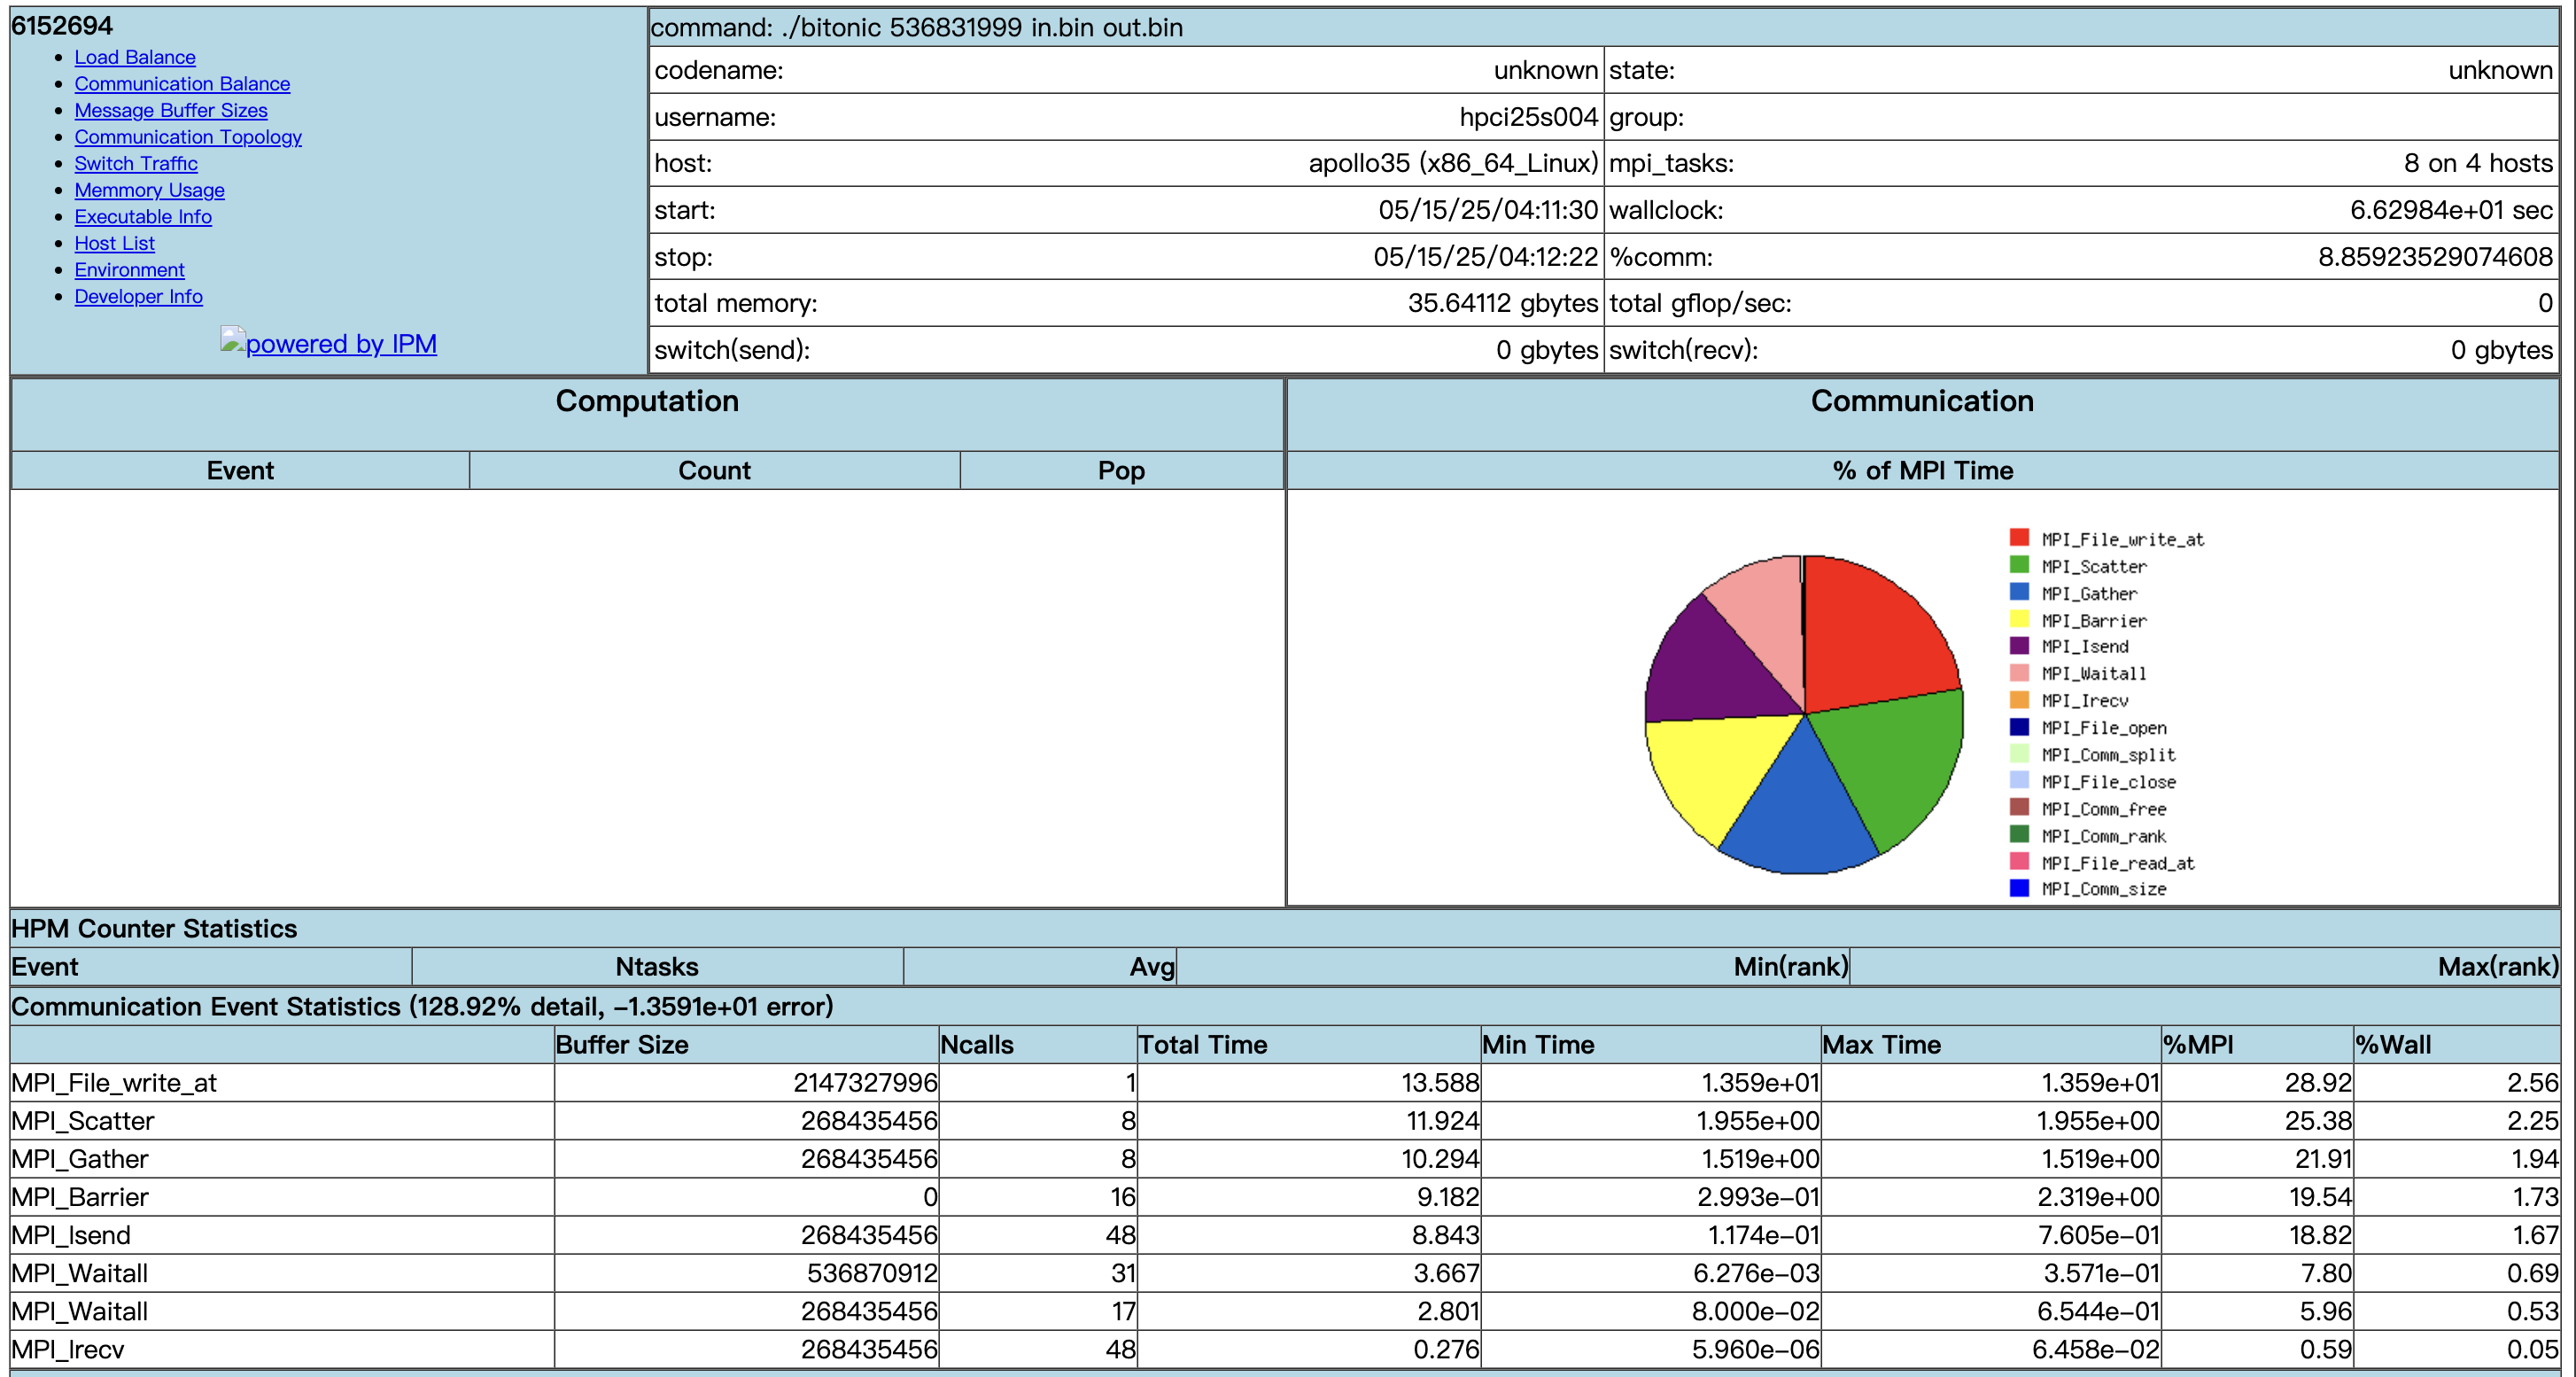
\includegraphics[width=1\textwidth]{./img/IPM.png}
    \caption{IPM Profile of MPI routines}
\end{figure}

\begin{table}[h!]
    \centering
    \begin{tabular}{lrr}
        \hline
        MPI Routine & \% of MPI & \% of Wall \\
        \hline
        MPI\_File\_write\_at & 28.92\% & 2.56\% \\
        MPI\_Scatter         & 25.38\% & 2.25\% \\
        MPI\_Gather          & 21.91\% & 1.95\% \\
        \hline
    \end{tabular}
    \caption{Top MPI routines by time share}
\end{table}

\section*{Future Optimisations}
\begin{enumerate}
    \item \textbf{Fully parallel I/O}: Replace rank-0 funnel with \texttt{MPI\_File\_read\_all} / \texttt{MPI\_File\_write\_all}.
    \item \textbf{Hybrid parallelism}: Overlap computation and communication by double-buffering \texttt{cmp} and using OpenMP within each rank.
    \item \textbf{Custom datatypes}: Use MPI derived datatypes to pack blocks and reduce scatter/gather overhead.
\end{enumerate}

\section*{Conclusion}
The implementation achieves correct global sorting with per-rank complexity
$\mathcal{O}(\tfrac{N}{p}\log^2\tfrac{N}{p})$ and scales up to 32 processes.
Serial I/O remains the performance bottleneck to address next.

\end{document}
